\addcontentsline{toc}{chapter}{Bezpieczeństwo i archiwizacja}
W czasach nieustannych wycieków danych i wciąż rosnącego cyberprzestępstwa istotnym elementem jest zapewnienie odpowiedniego poziomu bezpieczeństwa aplikacji. Według analizy przeprowadzonej przez "Rzeczpospolitą", która przedstawiono na rysunku 1 na podstawie informacji policji dotyczących incydentów związanych z oszustwami internetowymi oraz phisingiem, Czyli atakami polegającym na wyłudzaniu danych, \cite{phishing}  można stwierdzić, że w ciągu ostatnich pięciu lat liczba wykrytych w Polsce przestępstw cybernetycznych wzrosła o 72\% \cite{wykresbezpieczenstwo} [\ref{fig:Wykres}].

poprawic wykres i to jak wyglada
\begin{figure}[h]
	\centering
	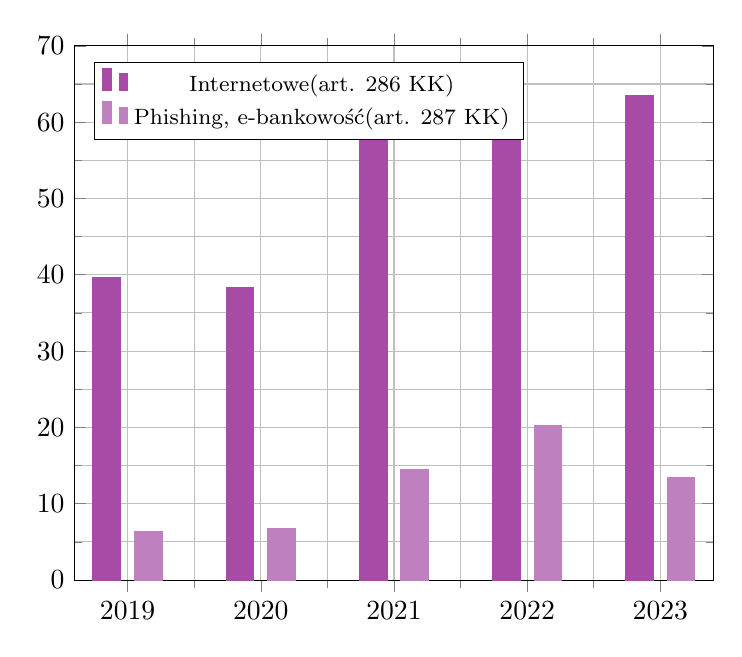
\begin{tikzpicture}
		\begin{axis}[
			symbolic x coords={2019,2020,2021,2022,2023},
			xtick=data,
			ymin=0, ymax=70,
			ytick={0,10,20,30,40,50,60, 70, 80, 90, 100},
			grid=both,
			minor tick num=1,
			width=0.8\textwidth, % szerokość wykresu jest 80% szerokości tekstu
			legend pos=north west, % pozycja legendy
			legend style={font=\footnotesize}, % wielkość czcionki legendy
			ybar=5pt, % szerokość słupków
			bar width=10pt, % szerokość pojedynczego słupka
			]
			\addplot[violet!70!white,fill=violet!70!white] coordinates {
				(2019, 39.6)
				(2020, 38.3)
				(2021, 59.1)
				(2022, 62.9)
				(2023, 63.5)
			};
			\addlegendentry{Internetowe(art. 286 KK)}

			\addplot[violet!50!white,fill=violet!50!white] coordinates {
				(2019, 6.3)
				(2020, 6.7)
				(2021, 14.5)
				(2022, 20.3)
				(2023, 13.4)
			};
			\addlegendentry{Phishing, e-bankowość(art. 287 KK)}
		\end{axis}
	\end{tikzpicture}
	\caption{Wykres przedstawiający dane( w tys.) internetowe i phishing, e-bankowość dla lat 2019-2023.}
	\label{fig:Wykres}
\end{figure}

\section*{Ukryte zmienne środowiskowe}
\addcontentsline{toc}{section}{Ukryte zmienne środowiskowe}

Aby chronić się przed atakami, które mogą prowadzić do przeciążenia bazy danych i uniemożliwienia dostęp użytkownikom do aplikacji, poprzez generowanie ogromnej ilości żądań HTTPS, należy korzystać z pliku .env. Plik ten umożliwia przekazywanie zmiennych środowiskowych w sposób tajny.

\begin{figure}[ht]
	\centering
	\vspace{0.25cm}
	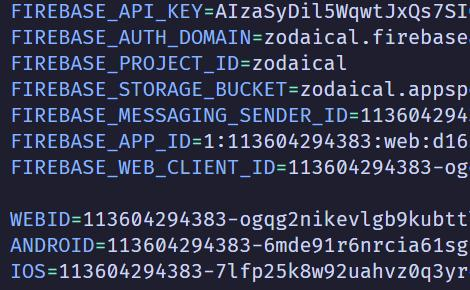
\includegraphics[height=7cm]{images/bezpieczenstwo/env}
	\caption{Zawartość pliku .env}
	\label{fig:Env}
\end{figure}

\newpage
W przypadku projektu ZodiaCal skorzystano ze zmiennych środowiskowych w pliku konfiguracyjnym Firebase, w plikach konfiguracyjnych do integracji zewnętrznych API obsługujących horoskop oraz bazę danych kosmetyków, w pliku SignIn ukrywając ID klienta potrzebnego do logowania się za pomocą konta Google oraz w miejscach w których skorzystano ze zdjęć z Firebase Storage (Rys.\ref{fig:FirebaseConfig}).

\begin{figure}[ht]
	\centering
	\vspace{0.25cm}
	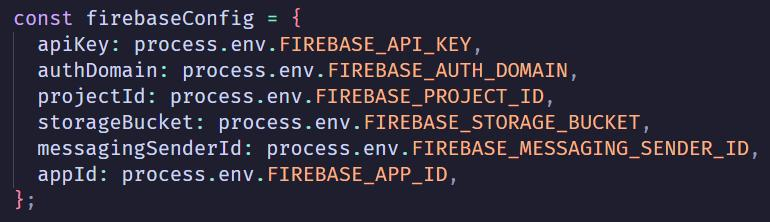
\includegraphics[height=4cm]{images/bezpieczenstwo/firebaseConfig}
	\caption{Wykorzystanie zmiennych globalnych w pliku konfiguracyjnym Firebase}
	\label{fig:FirebaseConfig}
\end{figure}

\section*{Walidacja formularzy}
\addcontentsline{toc}{section}{Walidacja formularzy}
Kluczowym sposobem na ochronę aplikacji przed atakami cybernetycznymi jest walidacja formularza. Pozwala ona na utrzymanie integralności danych i uniknięciu takich sytuacji, w których na przykład jeden użytkownik ma więcej, niż jedno konto przypisane do tego samego adresu e-mail. Można to osiągnąć korzystając z wbudowanych metodach Firebase odwołując się do komunikatu błędu „auth/email-already-in-use” tak jak jest to widoczne na rysunku \ref{fig:Auth}.

\begin{figure}[ht]
	\centering
	\vspace{0.25cm}
	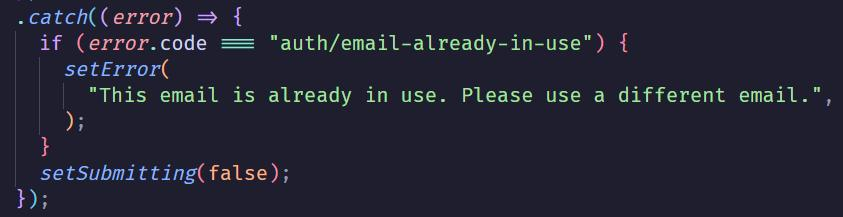
\includegraphics[height=4cm]{images/bezpieczenstwo/auth_email}
	\caption{Kod odpowiedzialny za weryfikację czy adres email jest już zapisany w bazie danych}
	\label{fig:Auth}
\end{figure}

Dodatkowo mechanizm wymuszający na klientach wprowadzenie silnego hasła, czyli takiego, który ma odpowiedną długość, posiada jedną wielką literę oraz znak specjalny, chroni konta użytkowników przed atakiem brute force polegającym na złamaniu hasła poprzez sprawdzanie przez algorytm wszystkich możliwych kombinacji tekstowych. Do weryfikacji, czy hasło zawiera specjalny znak skorzystano z wyrażenia regularnego, czyli ciąg znaków, który definiuje określony wzorzec.

\begin{figure}[ht]
	\centering
	\vspace{0.25cm}
	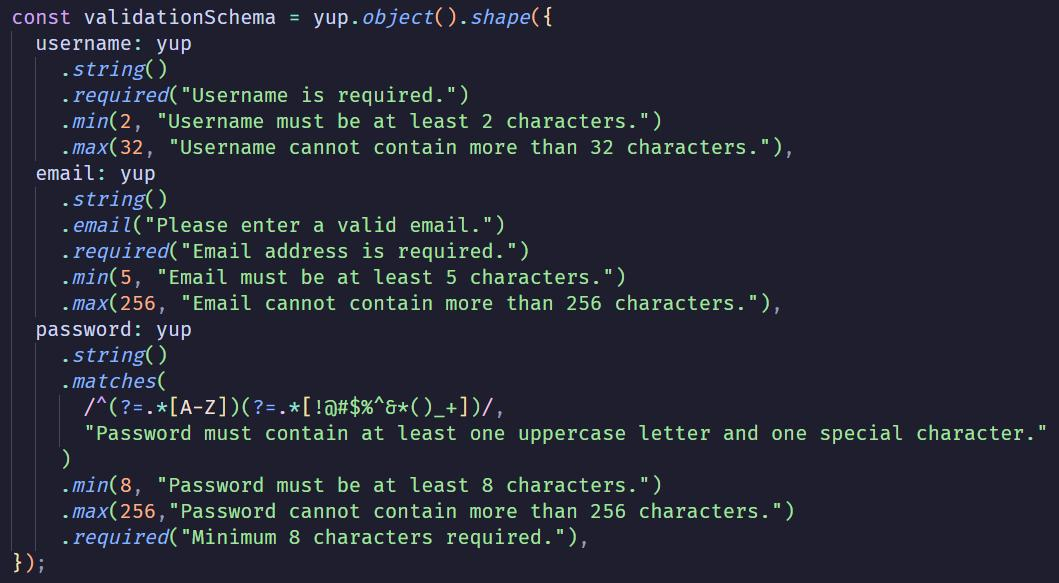
\includegraphics[height=8.5cm]{images/bezpieczenstwo/validationSchema}
	\caption{Kod odpowiedzialny za weryfikację czy adres email jest już zapisany w bazie danych}
	\label{fig:Validation}
\end{figure}

W celu osiągnięcia wyżej wymienionych korzyści wykorzystano bibliotekę yup, która pozwala zdefiniować wymagania pól tekstowych w formularzu poprzez ustalenie typu zmiennej wyjściowej, określenie czy pole jest obowiązkowe oraz ustalenie długości ciągów znaków co przedstawiono na rysunku (Rys.\ref{fig:Validation}). Podane wartości maksymalne zostały zdefiniowane przez dokument RFC 5321 \cite{rfc} definiujący standardy dotyczące protokołu używanego do przekazywania wiadomości e-mail. Ustalenie limitów pól formularza jest kluczowe, aby zapobiec problemom związanych z wydajnością systemu.

Dodatkowo każdy warunek powinien mieć unikalny komunikat błędu. Jest to korzystne zarówno dla dewelopera jak i użytkownika, ponieważ można określić w którym momencie pojawił się problem.


\section*{Ograniczona liczba prób logowania}
\addcontentsline{toc}{section}{Ograniczona liczba prób logowania}
Kolejnym sposobem na zapewnienie bezpieczeństwa aplikacji jest kontrola liczby prób logowania się do systemu. Kod na rysunku \ref{fig:LiczbaProb} zwiększa licznik prób logowania wykorzystując funkcję do aktualizacji stanu.

\begin{figure}[ht]
	\centering
	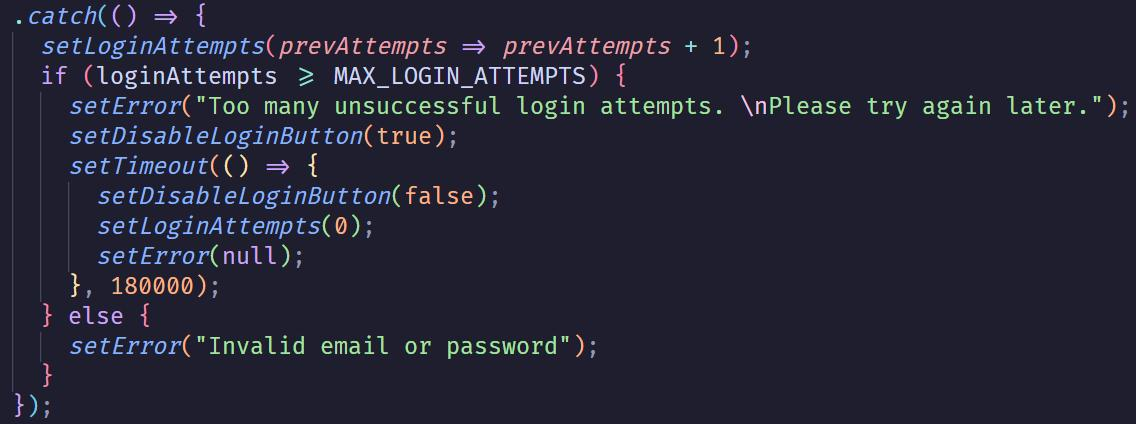
\includegraphics[height=6cm]{images/bezpieczenstwo/liczba_prob_kod}
	\caption{Fragment kodu odpowiadający za mechanizm zliczania prób logowania}
	\label{fig:LiczbaProb}
\end{figure}

 Następnie sprawdza, czy liczba prób przekracza wymaganą wartość. Jeśli tak, na ekranie pojawi się komunikat błędu, a przycisk logowania zostanie dezaktywowany (Rys.\ref{fig:Blad}). Użytkownik musi odczekać 3 minuty, po tym czasie licznik prób jest zerowany i można spróbować się zalogować.

\begin{figure}[ht]
	\centering
	\vspace{0.25cm}
	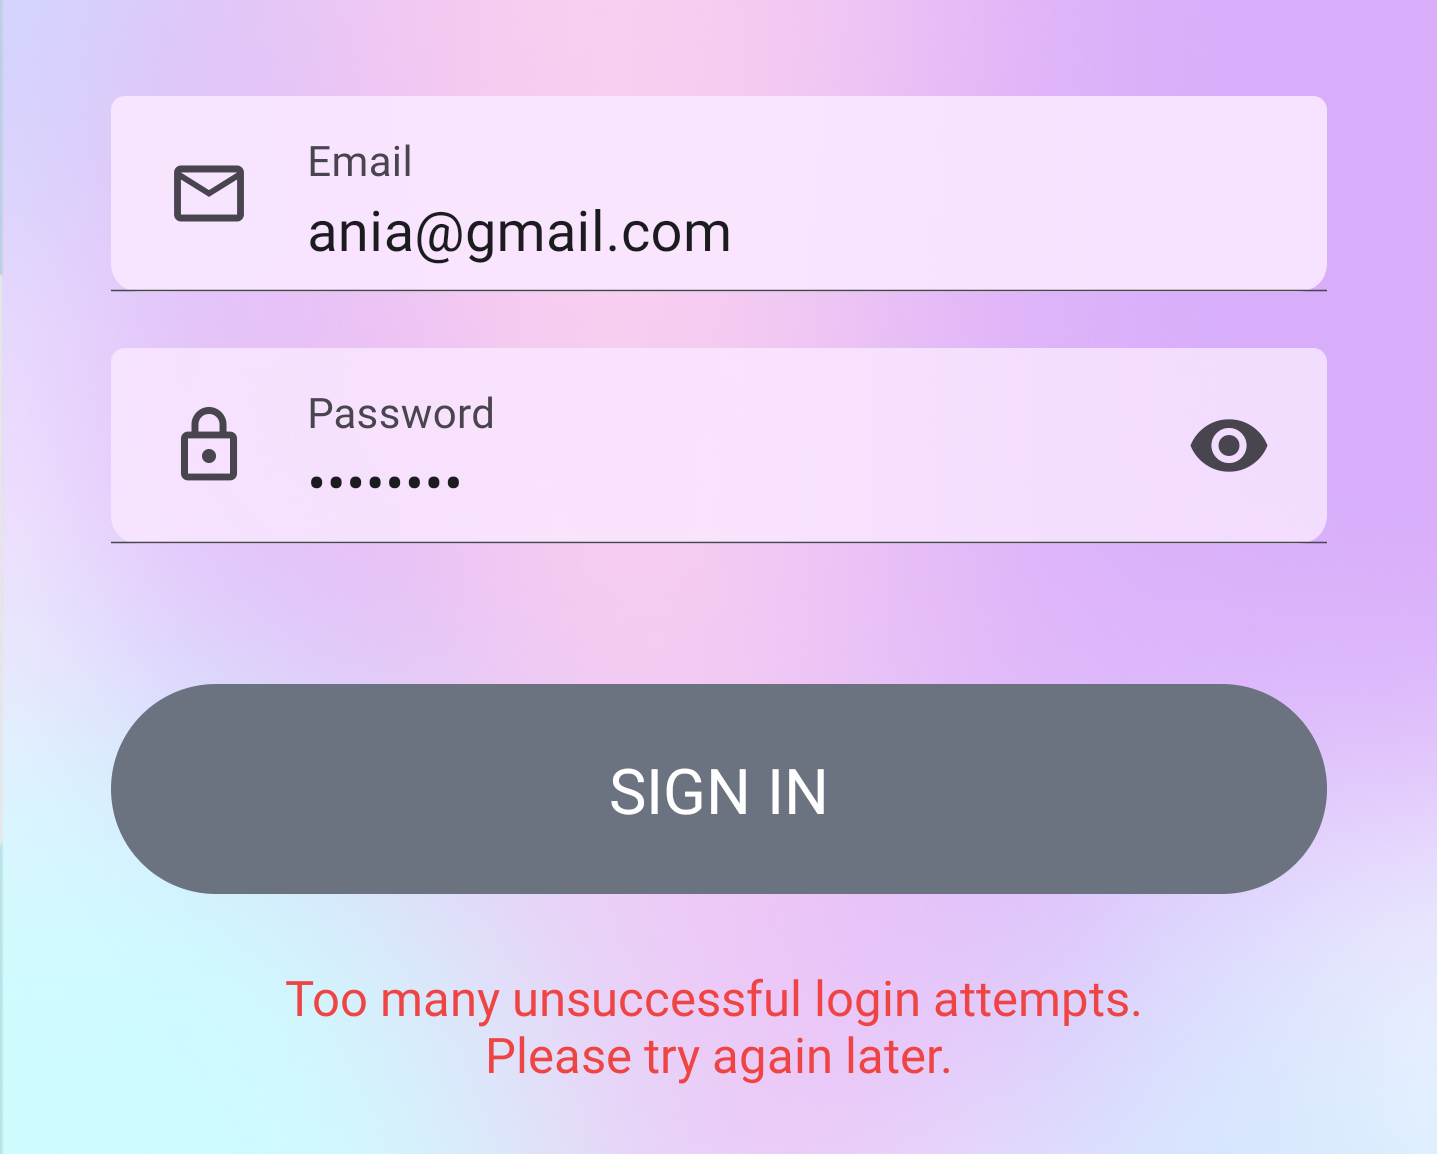
\includegraphics[height=6cm]{images/bezpieczenstwo/blad}
	\caption{Komunikat błędu na emulatorze}
	\label{fig:Blad}
\end{figure}

\section*{Zarządzanie sesją użytkownika}
\addcontentsline{toc}{section}{Zarządzanie sesją użytkownika}
Po uzupełnieniu pól tekstowych formularza i wciśnięciu przycisku logowania, dane są weryfikowane za pomocą metody signInWithEmailAndPassword dostarczonej przez Firebase. Jeśli zostały poprawnie wprowadzone użytkownik zmieni stan i zostaje przeniesiony do głównej części aplikacji.

Zarządzanie sesją użytkownika chroni przed nieautoryzowanym dostępem do zasobów aplikacji. Początkowo niezalogowany użytkownik ma dostęp jedynie do dwóch ekranów: SignIn oraz SignUp, natomiast po poprawnym zalogowaniu
i uwierzytelnieniu ma on dostęp do pełnej zawartości aplikacji.

Poniższy fragment kodu na rysunku \ref{fig:Blad} przedstawia nawigator, pełniący rolę kontrolera, który weryfikuje status zalogowania użytkownika i w oparciu o tę informację kieruje go między ekranami.

\begin{figure}[ht]
	\centering
	\vspace{0.25cm}
	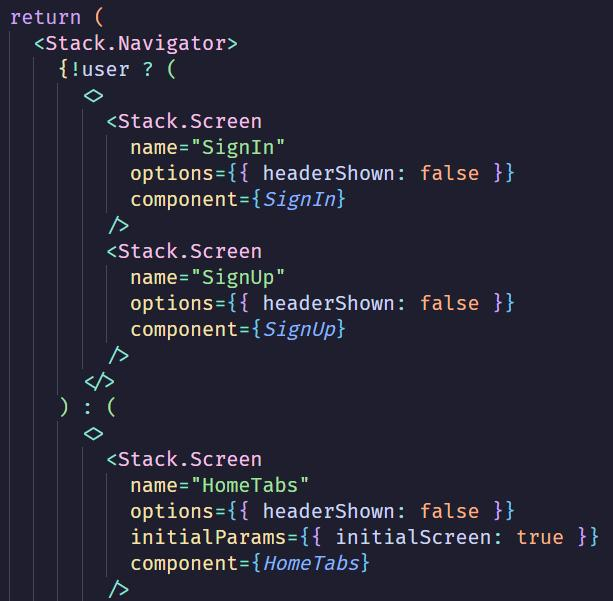
\includegraphics[height=9cm]{images/bezpieczenstwo/nawigator}
	\caption{Kod definiujący nawigację w zależności od stanu użytkownika}
	\label{fig:Nawigator}
\end{figure}


\section*{Archiwizacja}
\addcontentsline{toc}{section}{Archiwizacja}
Firebase zapewnia archiwizację bazy danych. Posiada narzędzia pozwalające na ręczne tworzenie kopii zapasowych oraz dodatkowo w płatnym planie Firebase cyklicznie, automatycznie tworzy kopie zapasowe. W przypadku aplikacji ZodiaCal kopia zapasowa bazy danych jest tworzone raz na miesiąc. Ta częstotliwość została ustalona na podstawie domyślnej konfiguracji Firebase oraz ograniczonych zasobów projektu.
Regularne kopie zapasowy usprawniają przywrócenie danych w przypadku ataku ransomware, polegającego na umyślnym zaszyfrowaniu lub uszkodzeniu bazy danych, w celu wymuszenia zapłaty okupu.

